\newpage
\section{Projective Geometry}

While people were still struggling with Euclid's postulate (until the
19th Century) the Renaissance was happening in Europe (15th Century).
In Italy this brought with it an interest in exploration and realism
in painting.  Realism demanded the understanding of perspective, that
is, how to faithfully represent the eye's view of a (3-dimensional)
landscape or other object extending off into the distance (two rails
of a train-track converging in the distance---small problem: There
were no railroads during the Renaissance).  Logical conclusion: There should
be a point infinitely far away where the two (parallel) rails meet.
In fact the geometers made those infinitely far away points.  Let's
see how.

The solid lines are the axes of 3-dimensional Euclidean space with
origin $O$.  The dotted plane is our canvas.
\[
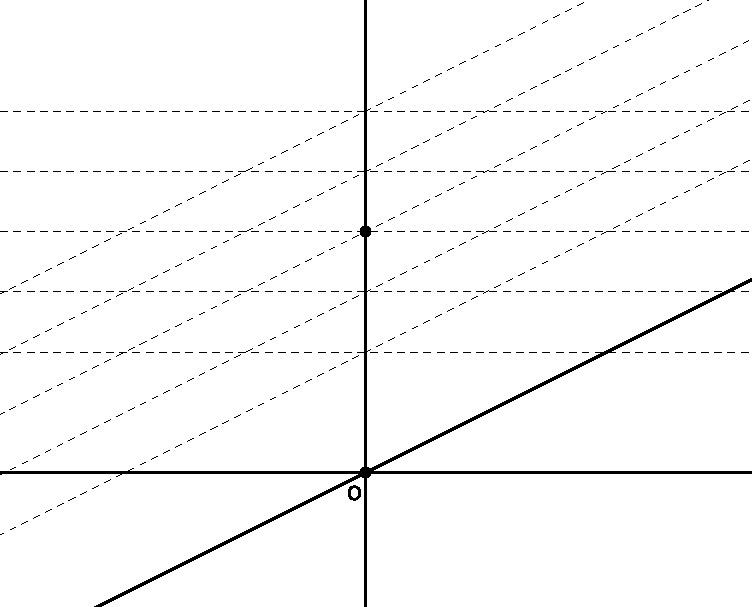
\includegraphics{../graphics/projPlane.pdf}
\]


\begin{prob} 
Put a point $A$ on the canvas.  Draw the line through $O$ and $A$ (and
extend it infinitely in both directions).
\end{prob}

\begin{prob} 
Put a point $B$ on the canvas.  Draw the line through $O$ and $B$ (and
extend it infinitely in both directions).
\end{prob}

\begin{prob} 
Does each point on the canvas determine a line through $O$?  Do
different points determine different lines through $O$?
\end{prob}

\begin{prob}\label{P:Start} 
Are there some lines through $O$ that get missed, that is, lines that
don't correspond to points on the canvas? Which ones?  We will say
that each of those lines corresponds to a `canvas point at infinity.'
\end{prob}

\begin{prob} 
Draw some train tracks (parallel lines $l$ and $m$) on the canvas.  Show
that each rail (line) determines a plane through $O$.
\end{prob}

\begin{prob}\label{P:Finish}
Let $L$ and $M$ stand for the planes through $O$ corresponding to the lines
$l$ and $m$ respectively.  How do $L$ and $M$ intersect?
\end{prob}

\begin{prob}
How do you find the line at which the planes $L$ and $M$ intersect?
\end{prob}

\begin{prob} 
Why do Problems \ref{P:Start} through \ref{P:Finish} above justify the
statement that ``parallel lines on the canvas also meet at exactly one
point, it's just that point is a canvas point at infinity?''
\end{prob}




